% Owner: Vikash Kumar. Results: performance analysis, CPI/IPC, speed-up and waveforms.
% Every metric below comes directly from analysis/results/perf.csv,
% analysis/results/speedup.csv, and synth/reports/summary.csv.
\subsection{Performance Analysis}
\label{sec:perf}

This subsection evaluates the cycle efficiency, instruction throughput, execution time,
and net speed-up of the 5-stage pipelined processor in comparison to the single-cycle
baseline. All measurements are derived from cycle-accurate Verilog simulations executed
via \texttt{analysis/run\_perf.sh} and static timing analysis from the FPGA synthesis
reports (\S\ref{sec:synth}).

\subsubsection{Cycle Count Model and Validation}
In an ideal five-stage pipeline without hazards, one instruction completes every clock
cycle after an initial four-cycle pipeline fill latency ($C = N + 4$, yielding
$\text{CPI} \to 1.0$ for large $N$)~\cite{vikashPattersonRV}. However, data and control
hazards introduce cycle penalties:
\begin{itemize}
  \item \textbf{Load-Use Hazard Stall ($S$ cycles):} A load instruction followed
        immediately by a dependent instruction cannot be resolved solely by forwarding,
        because the loaded memory data is not available until the end of the MEM stage.
        The hazard detection unit inserts one bubble ($S = 1$ cycle per hazard).
  \item \textbf{Branch / Jump Flush ($2T$ cycles):} Under the predict-not-taken policy,
        conditional branches and unconditional jumps evaluate in the EX stage. If taken,
        the two instructions speculatively fetched into IF/ID and ID/EX are flushed
        ($2$ bubbles per taken transfer, $2T$ cycles in total).
\end{itemize}
The total execution cycles $C$ from reset deassertion until the final \texttt{jal x0, 0}
halt completes write-back is governed by the analytical equation:
\begin{equation}
  C_{\text{pipeline}} = N + 4 + S + 2T
  \label{eq:cycles}
\end{equation}
For the single-cycle baseline, every instruction completes in exactly one long clock
cycle, giving $C_{\text{single}} = N$, $\text{CPI} = 1.000$, and $\text{IPC} = 1.000$
with $S = 0$ and $T = 0$.

Table~\ref{tab:perf_summary} reports the measured execution metrics across all six Phase~I
system test programs and six Phase~II realistic benchmarks. In every single test and
benchmark run, the simulated cycle count $C_{\text{pipeline}}$ matches
Equation~\eqref{eq:cycles} with zero discrepancy, validating the cycle-accurate behavior
of the hazard detection and forwarding units.

\begin{table*}[!t]
\centering
\caption{Cycle-Accurate Performance Comparison: Single-Cycle Baseline vs. 5-Stage Pipeline}
\label{tab:perf_summary}
\setlength{\tabcolsep}{4.5pt}
\renewcommand{\arraystretch}{1.1}
\begin{tabular}{@{}lrrrrrrrrr@{}}
\toprule
 & \multicolumn{3}{c}{\textbf{Single-Cycle Baseline}} & \multicolumn{6}{c}{\textbf{5-Stage Pipelined Processor}} \\
\cmidrule(lr){2-4} \cmidrule(lr){5-10}
\textbf{Program} & \textbf{$N$} & \textbf{Cycles ($C$)} & \textbf{CPI} & \textbf{Cycles ($C$)} & \textbf{Stalls ($S$)} & \textbf{Taken ($T$)} & \textbf{CPI} & \textbf{IPC} & \textbf{$N+4+S+2T$} \\
\midrule
\texttt{test1\_arith}       & 21   & 21   & 1.000 & 25   & 0   & 0   & 1.190 & 0.840 & $21+4+0+0 = 25$ \\
\texttt{test2\_loadstore}   & 7    & 7    & 1.000 & 11   & 0   & 0   & 1.571 & 0.636 & $7+4+0+0 = 11$ \\
\texttt{test3\_forwarding}  & 6    & 6    & 1.000 & 10   & 0   & 0   & 1.667 & 0.600 & $6+4+0+0 = 10$ \\
\texttt{test4\_loaduse}     & 5    & 5    & 1.000 & 10   & 1   & 0   & 2.000 & 0.500 & $5+4+1+0 = 10$ \\
\texttt{test5\_branch\_jump}& 11   & 11   & 1.000 & 23   & 0   & 4   & 2.091 & 0.478 & $11+4+0+8 = 23$ \\
\texttt{test6\_sum\_array}  & 40   & 40   & 1.000 & 57   & 5   & 4   & 1.425 & 0.702 & $40+4+5+8 = 57$ \\
\midrule
\texttt{bench\_fib}         & 785  & 785  & 1.000 & 1095 & 0   & 153 & 1.395 & 0.717 & $785+4+0+306 = 1095$ \\
\texttt{bench\_sum}         & 330  & 330  & 1.000 & 490  & 32  & 62  & 1.485 & 0.673 & $330+4+32+124 = 490$ \\
\texttt{bench\_sort}        & 920  & 920  & 1.000 & 1444 & 120 & 200 & 1.570 & 0.637 & $920+4+120+400 = 1444$ \\
\texttt{bench\_gcd}         & 786  & 786  & 1.000 & 1238 & 0   & 224 & 1.575 & 0.635 & $786+4+0+448 = 1238$ \\
\texttt{bench\_memcpy}      & 1231 & 1231 & 1.000 & 1741 & 128 & 189 & 1.414 & 0.707 & $1231+4+128+378 = 1741$ \\
\texttt{bench\_mul}         & 570  & 570  & 1.000 & 828  & 0   & 127 & 1.453 & 0.688 & $570+4+0+254 = 828$ \\
\bottomrule
\end{tabular}
\end{table*}

\subsubsection{Benchmark Cycle Breakdown and Hazard Characteristics}
Fig.~\ref{fig:cycle_breakdown} illustrates the composition of pipeline cycles for the
six realistic benchmarks, decomposing total cycles into instruction base execution ($N$),
pipeline startup fill ($4$ cycles), load-use stall cycles ($S$), and branch/jump flush
penalties ($2T$).

\begin{figure}[!t]
\centering
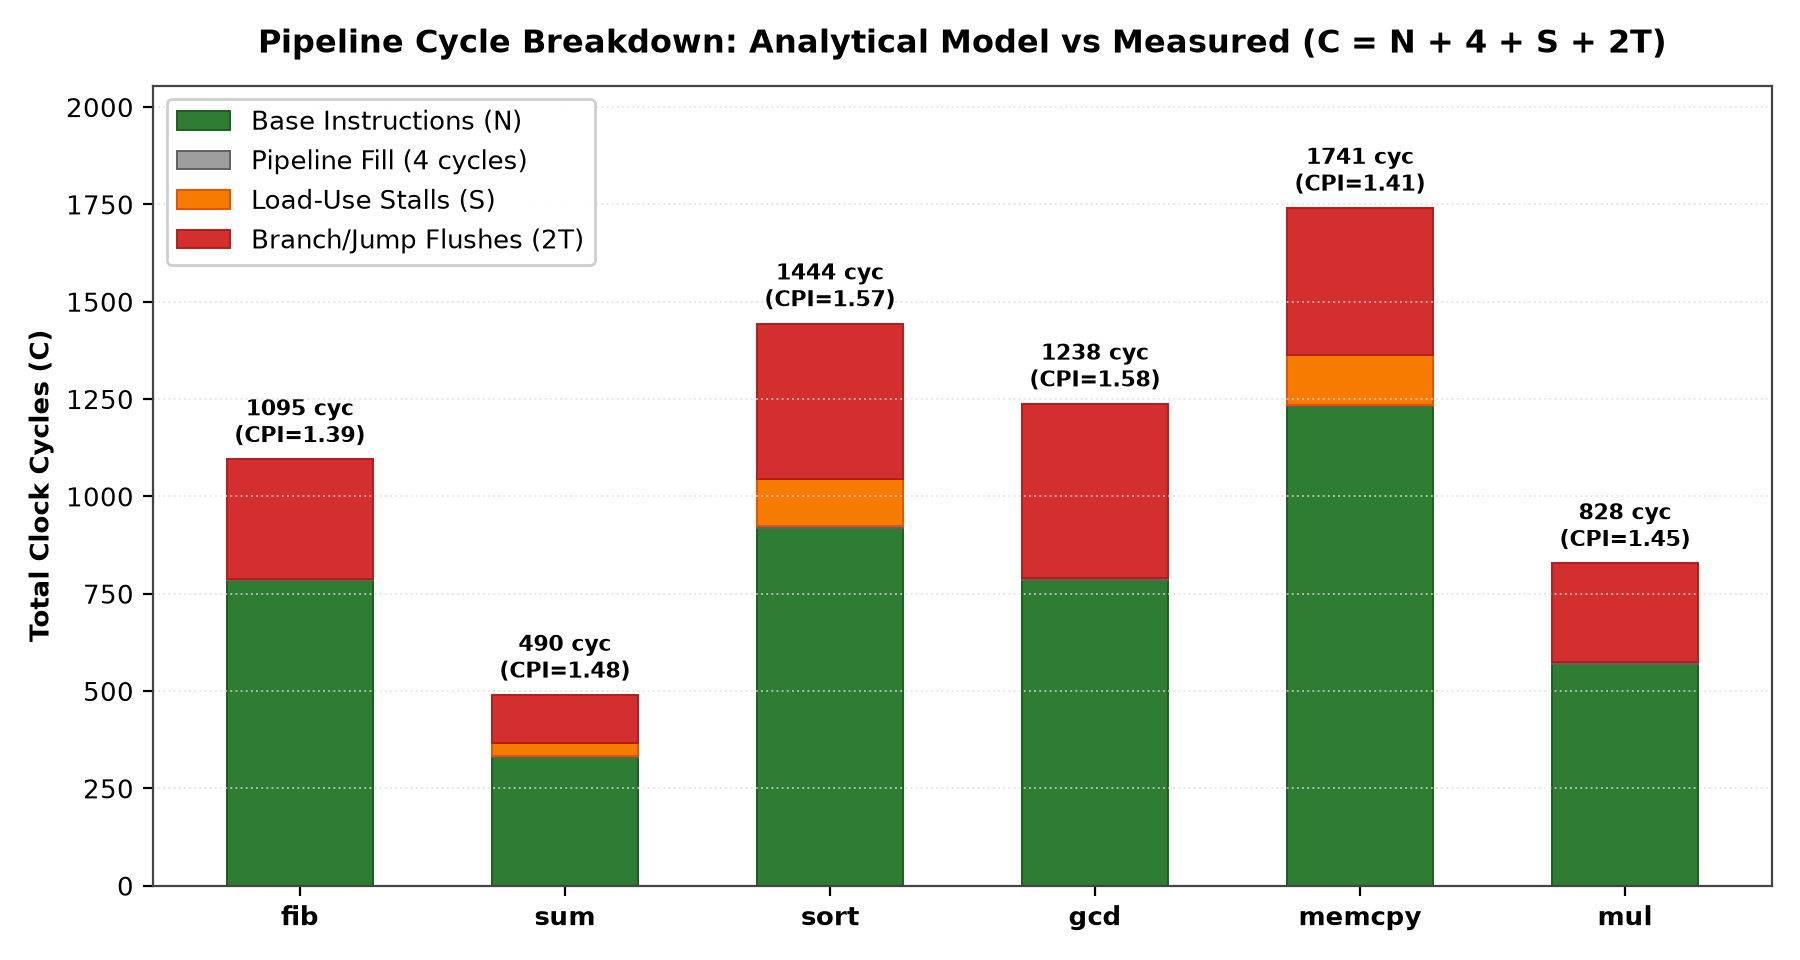
\includegraphics[width=\columnwidth]{analysis/figures/pipeline_cycle_breakdown.png}
\caption{Stacked pipeline cycle breakdown across Phase~II benchmarks ($C = N + 4 + S + 2T$),
showing the impact of load-use stalls ($S$) and taken branch/jump flushes ($2T$).}
\label{fig:cycle_breakdown}
\end{figure}

The distribution of hazards varies significantly across workloads:
\begin{enumerate}
  \item \textbf{Branch-Heavy Workloads (\texttt{bench\_gcd} and \texttt{bench\_fib}):}
        \texttt{bench\_gcd} exhibits the highest CPI ($1.575$) among all benchmarks.
        Implementing Euclid's subtraction-based algorithm, it contains multiple conditional
        branches per iteration. Over 786 executed instructions, $T = 224$ branches are
        taken, incurring $2 \times 224 = 448$ flush cycles (accounting for $36.2\,\%$ of
        total runtime). Because all data dependences involve registers and are resolved
        instantly by the forwarding unit, there are zero load-use stalls ($S = 0$).
        Similarly, \texttt{bench\_fib} has $S = 0$ and $T = 153$, achieving a lower
        CPI of $1.395$ due to a longer compute path per loop iteration.
  \item \textbf{Memory and Stall-Heavy Workloads (\texttt{bench\_sort} and \texttt{bench\_memcpy}):}
        \texttt{bench\_sort} (bubble sort) incurs both types of hazards in substantial
        quantities: $S = 120$ load-use stalls occur because the inner loop compares array
        elements immediately after loading them (\texttt{lw x14, 4(x11)} followed by
        \texttt{bge x14, x13, noswap}), while $T = 200$ taken branches add 400 flush
        cycles, resulting in $\text{CPI} = 1.570$. \texttt{bench\_memcpy} copies 64 words
        and computes verification checksums; back-to-back load-to-store operations and
        accumulations cause $S = 128$ stalls, yet its high instruction volume ($N = 1231$)
        dilutes the overhead to a competitive $\text{CPI} = 1.414$.
  \item \textbf{Array Traversal and Arithmetic (\texttt{bench\_sum} and \texttt{bench\_mul}):}
        \texttt{bench\_sum} executes $32$ load-use stalls on consecutive array loads,
        achieving $\text{CPI} = 1.485$. \texttt{bench\_mul} emulates 32-bit multiplication
        via shift-and-add; because operands reside in registers, $S = 0$, and data-dependent
        shifts yield $\text{CPI} = 1.453$.
\end{enumerate}

\begin{figure}[!t]
\centering
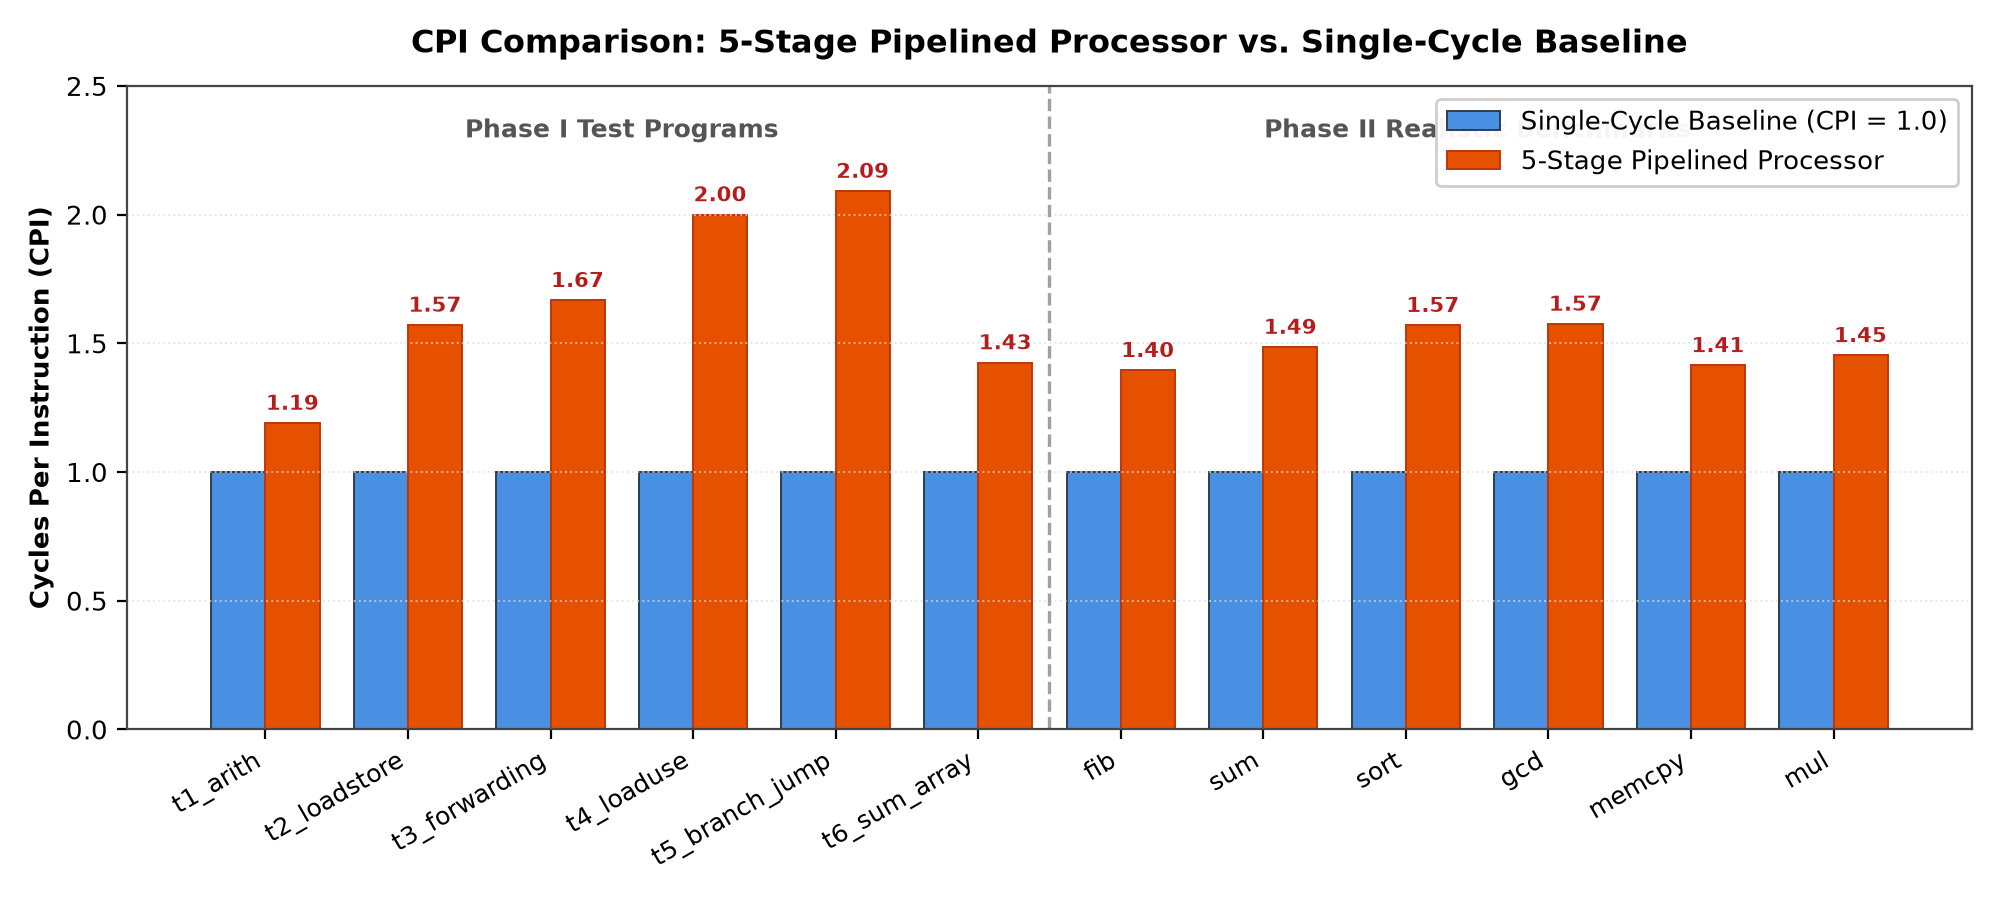
\includegraphics[width=\columnwidth]{analysis/figures/cpi_comparison.png}
\caption{Measured CPI comparison between the single-cycle baseline ($\text{CPI} = 1.0$)
and the 5-stage pipeline across all 12 programs.}
\label{fig:cpi_comp}
\end{figure}

\subsubsection{Execution Time and Speed-Up Analysis}
Although the single-cycle processor achieves $\text{CPI} = 1.000$, its maximum operating
frequency on the Lattice ECP5 FPGA is severely constrained by its unpipelined critical
path ($F_{\text{max}} = 28.43\,\text{MHz}$, $\S\ref{sec:synth}$). In contrast, the five-stage
pipeline partitions the critical path into shorter, balanced stages, achieving
$F_{\text{max}} = 56.55\,\text{MHz}$---a clock frequency increase of $1.9891\times$
($\approx 1.99\times$).

The wall-clock execution time for each architecture is given by:
\begin{equation}
  T_{\text{exec}} = \frac{C}{F_{\text{max}}}
\end{equation}
The true system speed-up of the pipeline over the single-cycle baseline is the ratio of
their execution times, which decomposes mathematically into the product of the cycle
ratio and the clock frequency ratio~\cite{vikashHennessyQA}:
\begin{equation}
  \text{Speed-Up} = \frac{T_{\text{single}}}{T_{\text{pipeline}}}
  = \left(\frac{C_{\text{single}}}{C_{\text{pipeline}}}\right) \times \left(\frac{F_{\text{max, pipe}}}{F_{\text{max, single}}}\right)
  = \left(\frac{1}{\text{CPI}_{\text{pipeline}}}\right) \times 1.9891
  \label{eq:speedup}
\end{equation}
Table~\ref{tab:speedup} presents the measured execution times and speed-up factors for all
workloads. Fig.~\ref{fig:exec_speedup} contrasts execution times and visualizes the
achieved speed-up.

\begin{table}[!t]
\centering
\caption{Execution Time and Speed-Up Comparison ($F_{\text{max}}$: Single = 28.43~MHz, Pipeline = 56.55~MHz)}
\label{tab:speedup}
\setlength{\tabcolsep}{4.5pt}
\renewcommand{\arraystretch}{1.1}
\begin{tabular}{@{}lrrrrr@{}}
\toprule
\textbf{Program} & \textbf{Time$_{\text{single}}$} & \textbf{Time$_{\text{pipe}}$} & \textbf{Cycle Ratio} & \textbf{$F_{\text{max}}$ Ratio} & \textbf{Speed-Up} \\
\midrule
\texttt{test1\_arith}       & 0.74\,\textmu s  & 0.44\,\textmu s  & 0.8400 & 1.9891 & $1.67\times$ \\
\texttt{test2\_loadstore}   & 0.25\,\textmu s  & 0.20\,\textmu s  & 0.6364 & 1.9891 & $1.27\times$ \\
\texttt{test3\_forwarding}  & 0.21\,\textmu s  & 0.18\,\textmu s  & 0.6000 & 1.9891 & $1.19\times$ \\
\texttt{test4\_loaduse}     & 0.18\,\textmu s  & 0.18\,\textmu s  & 0.5000 & 1.9891 & $0.99\times$ \\
\texttt{test5\_branch\_jump}& 0.39\,\textmu s  & 0.41\,\textmu s  & 0.4783 & 1.9891 & $0.95\times$ \\
\texttt{test6\_sum\_array}  & 1.41\,\textmu s  & 1.01\,\textmu s  & 0.7018 & 1.9891 & $1.40\times$ \\
\midrule
\texttt{bench\_fib}         & 27.61\,\textmu s & 19.36\,\textmu s & 0.7169 & 1.9891 & $\mathbf{1.43\times}$ \\
\texttt{bench\_sum}         & 11.61\,\textmu s & 8.67\,\textmu s  & 0.6735 & 1.9891 & $\mathbf{1.34\times}$ \\
\texttt{bench\_sort}        & 32.36\,\textmu s & 25.54\,\textmu s & 0.6371 & 1.9891 & $\mathbf{1.27\times}$ \\
\texttt{bench\_gcd}         & 27.65\,\textmu s & 21.89\,\textmu s & 0.6349 & 1.9891 & $\mathbf{1.26\times}$ \\
\texttt{bench\_memcpy}      & 43.30\,\textmu s & 30.79\,\textmu s & 0.7071 & 1.9891 & $\mathbf{1.41\times}$ \\
\texttt{bench\_mul}         & 20.05\,\textmu s & 14.64\,\textmu s & 0.6884 & 1.9891 & $\mathbf{1.37\times}$ \\
\bottomrule
\end{tabular}
\end{table}

\begin{figure}[!t]
\centering
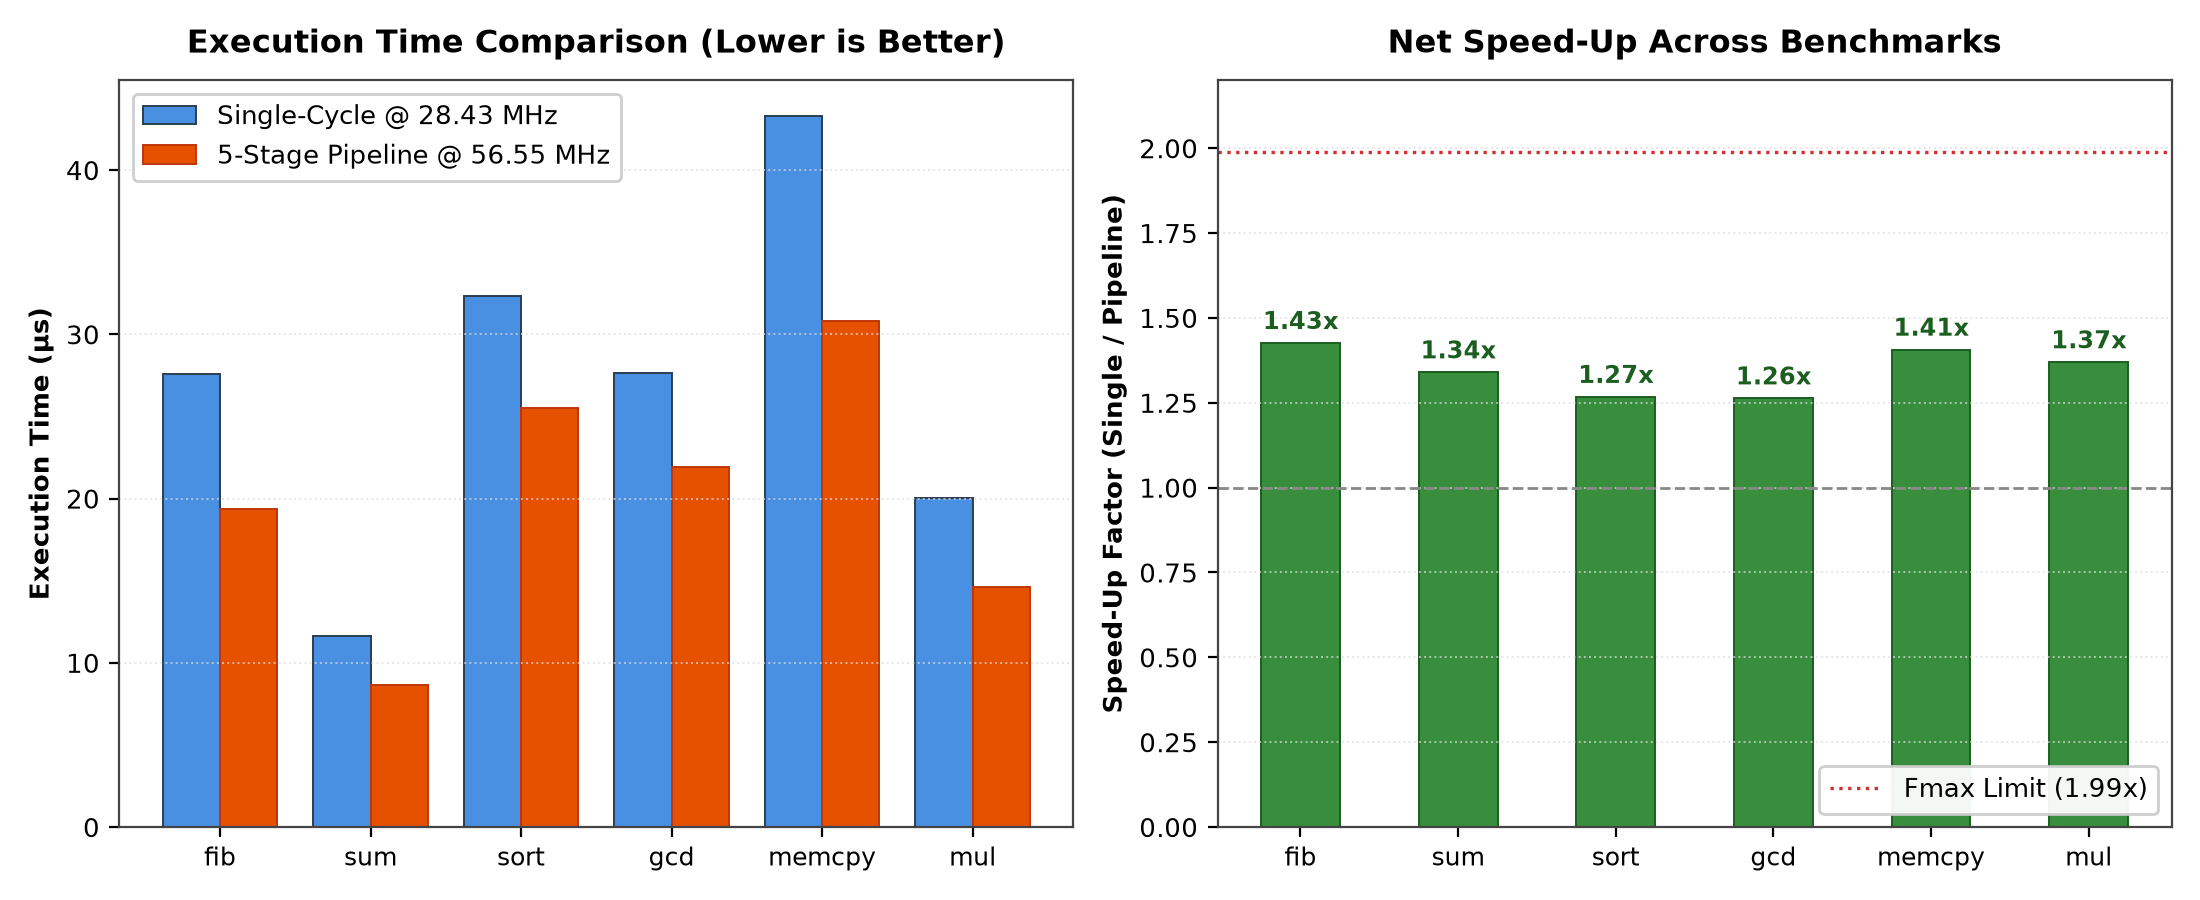
\includegraphics[width=\columnwidth]{analysis/figures/execution_time_speedup.png}
\caption{Comparison of execution times (left) and net speed-up factors (right)
across the realistic benchmark programs.}
\label{fig:exec_speedup}
\end{figure}

\subsubsection{Architectural Discussion}
Several key architectural conclusions arise from these results:
\begin{itemize}
  \item \textbf{Why Speed-Up is Below $5\times$:} A textbook five-stage pipeline
        theoretically offers up to a $5\times$ speed-up under zero hazard overhead and
        perfect stage delay balancing. In physical FPGA hardware, the speed-up is
        $1.26\times$ to $1.43\times$ due to two physical realities:
        (1)~The clock frequency scales by $1.99\times$ rather than $5\times$ because
        register setup times, clock-to-out delays, and FPGA routing overhead prevent
        dividing total latency into five equal slices.
        (2)~Pipeline hazards increase CPI from $1.000$ to $1.40$--$1.57$, which consumes
        approximately $28\,\%$ to $36\,\%$ of the frequency gains.
  \item \textbf{Amortization of Startup Overhead:} In short microbenchmarks such as
        \texttt{test4\_loaduse} ($N=5$) and \texttt{test5\_branch\_jump} ($N=11$), the
        four-cycle pipeline fill latency constitutes a massive fraction of execution time
        ($80\,\%$ and $36\,\%$, respectively), driving speed-up slightly below unity
        ($0.95\times$--$0.99\times$). In contrast, for realistic benchmark programs with
        hundreds of instructions, the fill overhead amortizes to less than $1.2\,\%$ of
        total execution, consistently delivering a solid $26\,\%$ to $43\,\%$ performance
        advantage.
  \item \textbf{Frequency Advantage Overcomes CPI Deficit:} Across all realistic benchmarks,
        the frequency multiplier ($1.9891\times$) comfortably exceeds the CPI degradation
        factor ($\text{CPI} \le 1.575$), proving that pipelining provides substantial
        net performance gains even on FPGA architectures where BRAM and distributed memory
        accesses dominate critical paths.
\end{itemize}

\subsubsection{GTKWave Waveform Verification}
To demonstrate cycle-accurate hardware verification, simulation traces were recorded in
VCD format and inspected in GTKWave~\cite{vikashBybellGTKWave}. The exact signal setups
are preserved in \texttt{simulation/gtkwave/*.gtkw} for full reproducibility.

\begin{figure*}[!t]
\centering
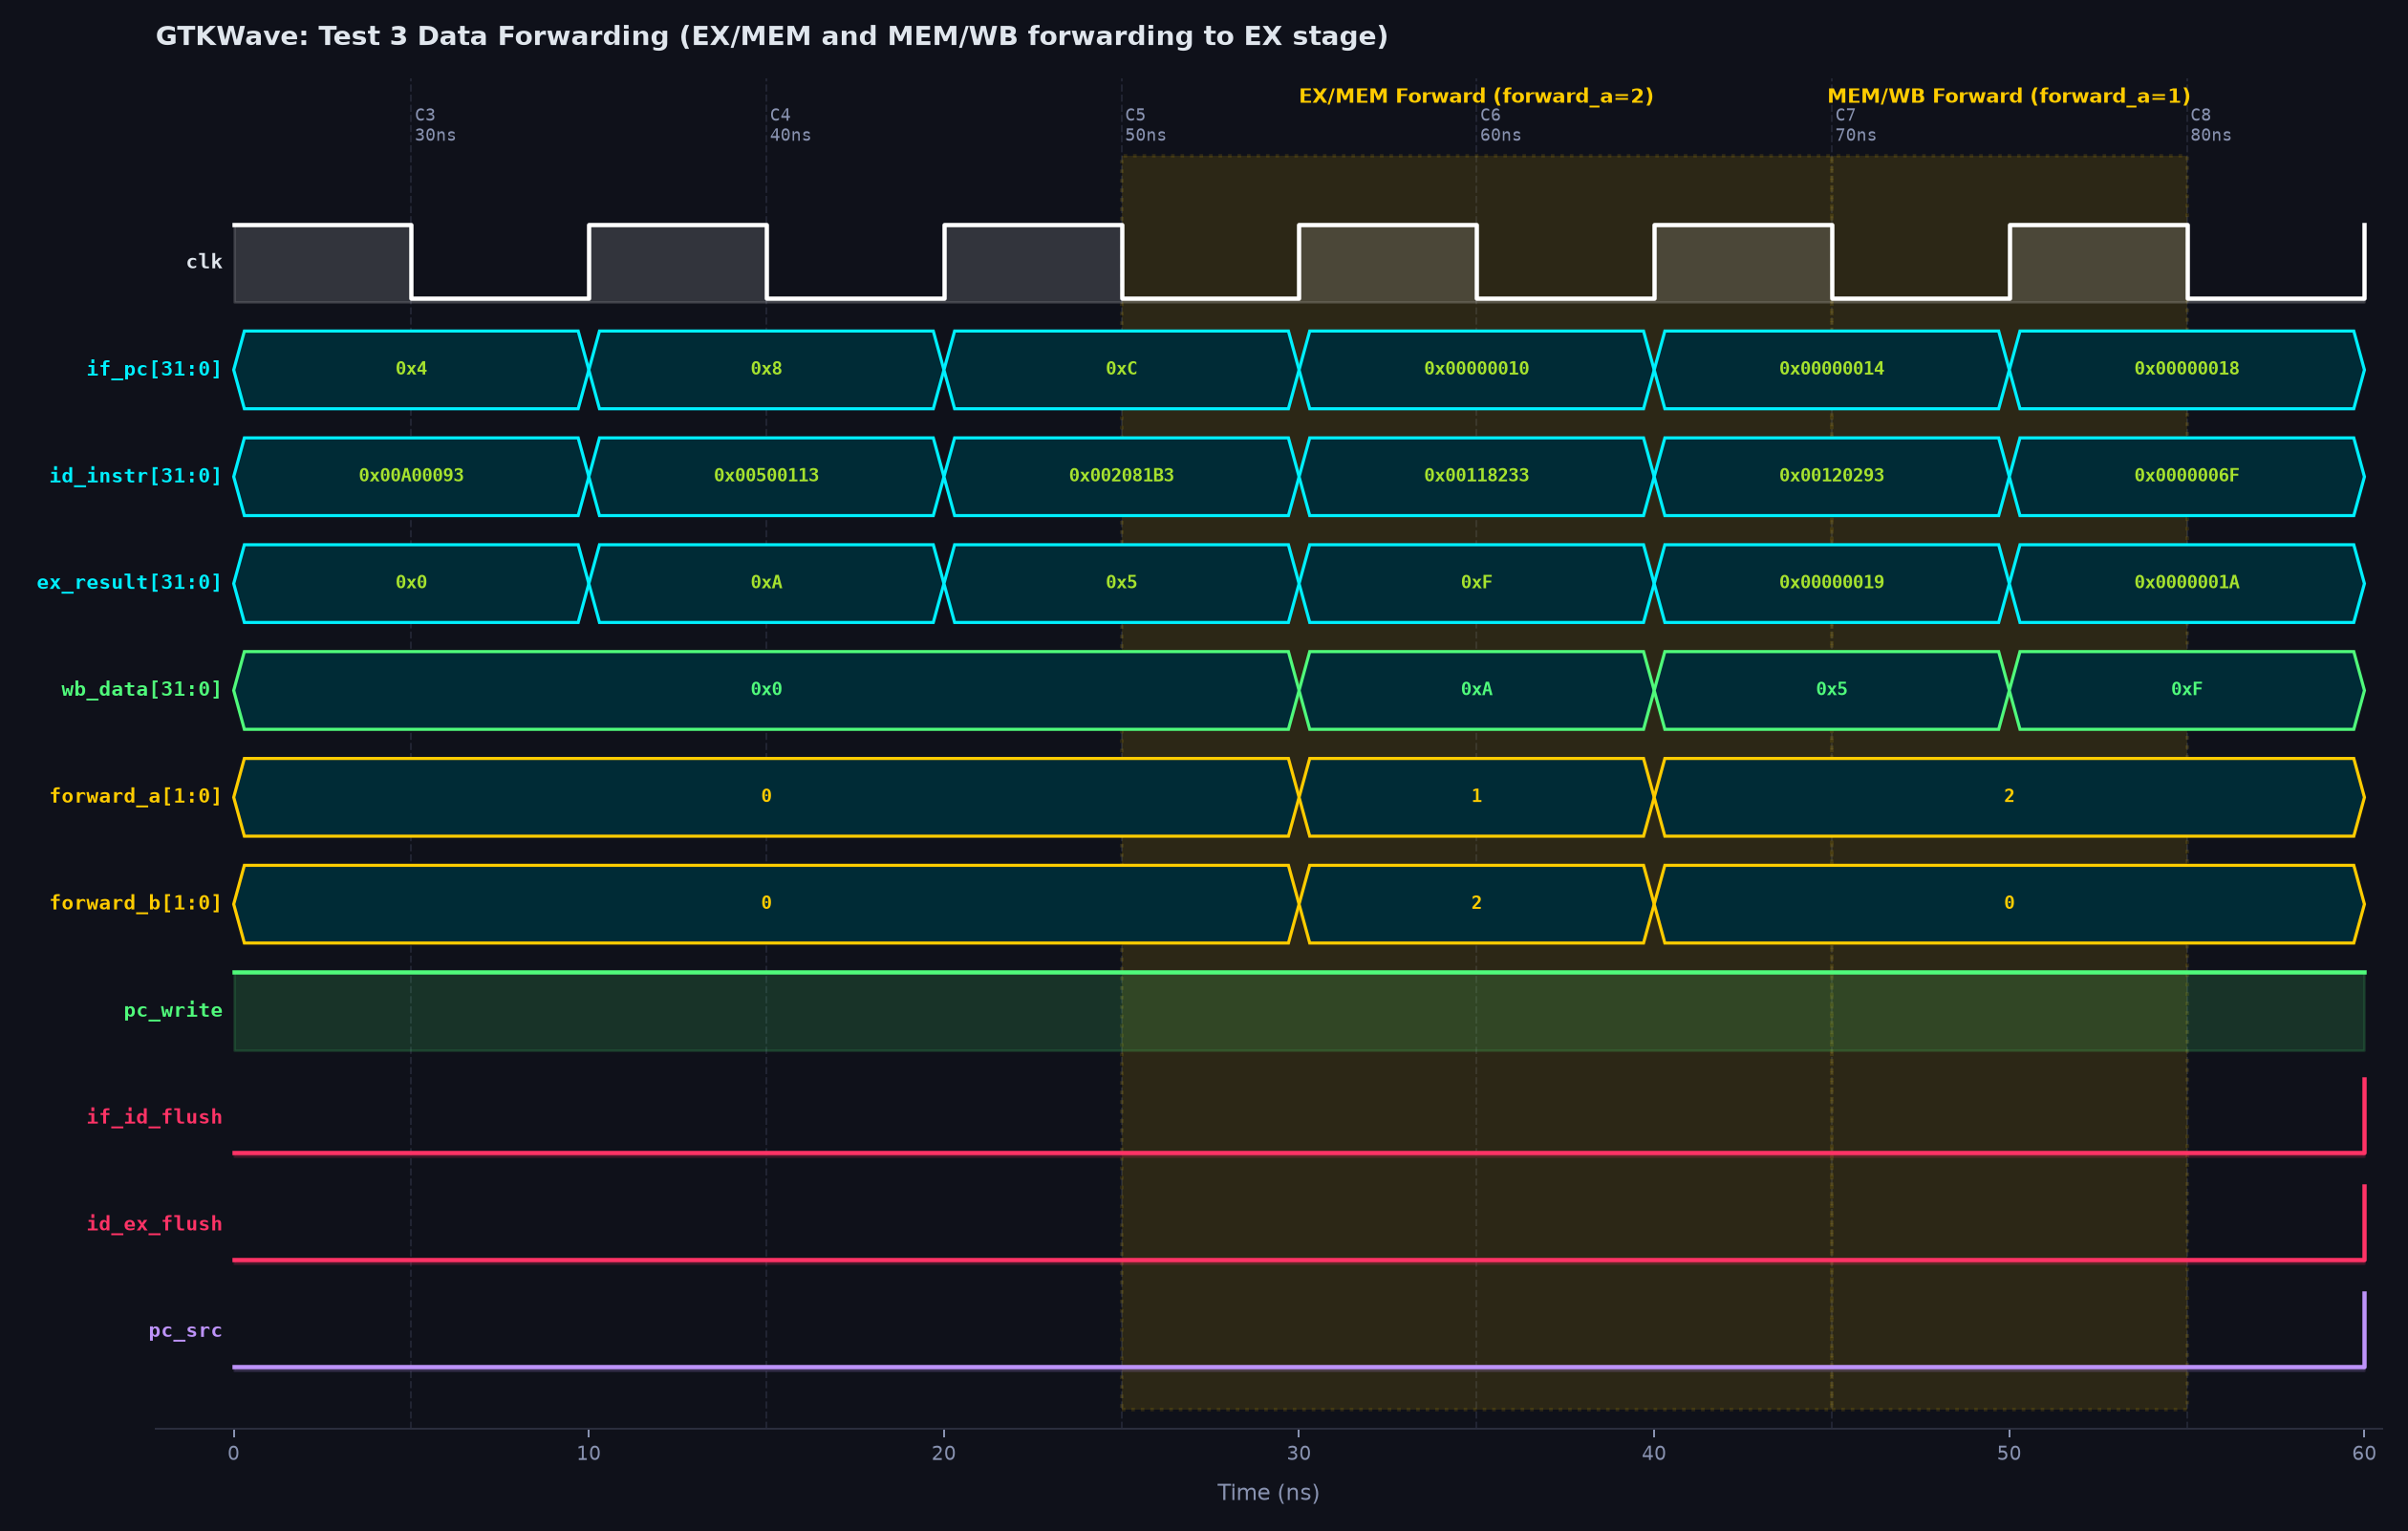
\includegraphics[width=0.92\textwidth]{diagrams/waveforms/forwarding.png}
\caption{GTKWave simulation waveform of System Test~3 (\texttt{test3\_forwarding}),
demonstrating back-to-back EX/MEM and MEM/WB data forwarding to the ALU inputs.}
\label{fig:wave_fwd}
\end{figure*}

\begin{figure*}[!t]
\centering
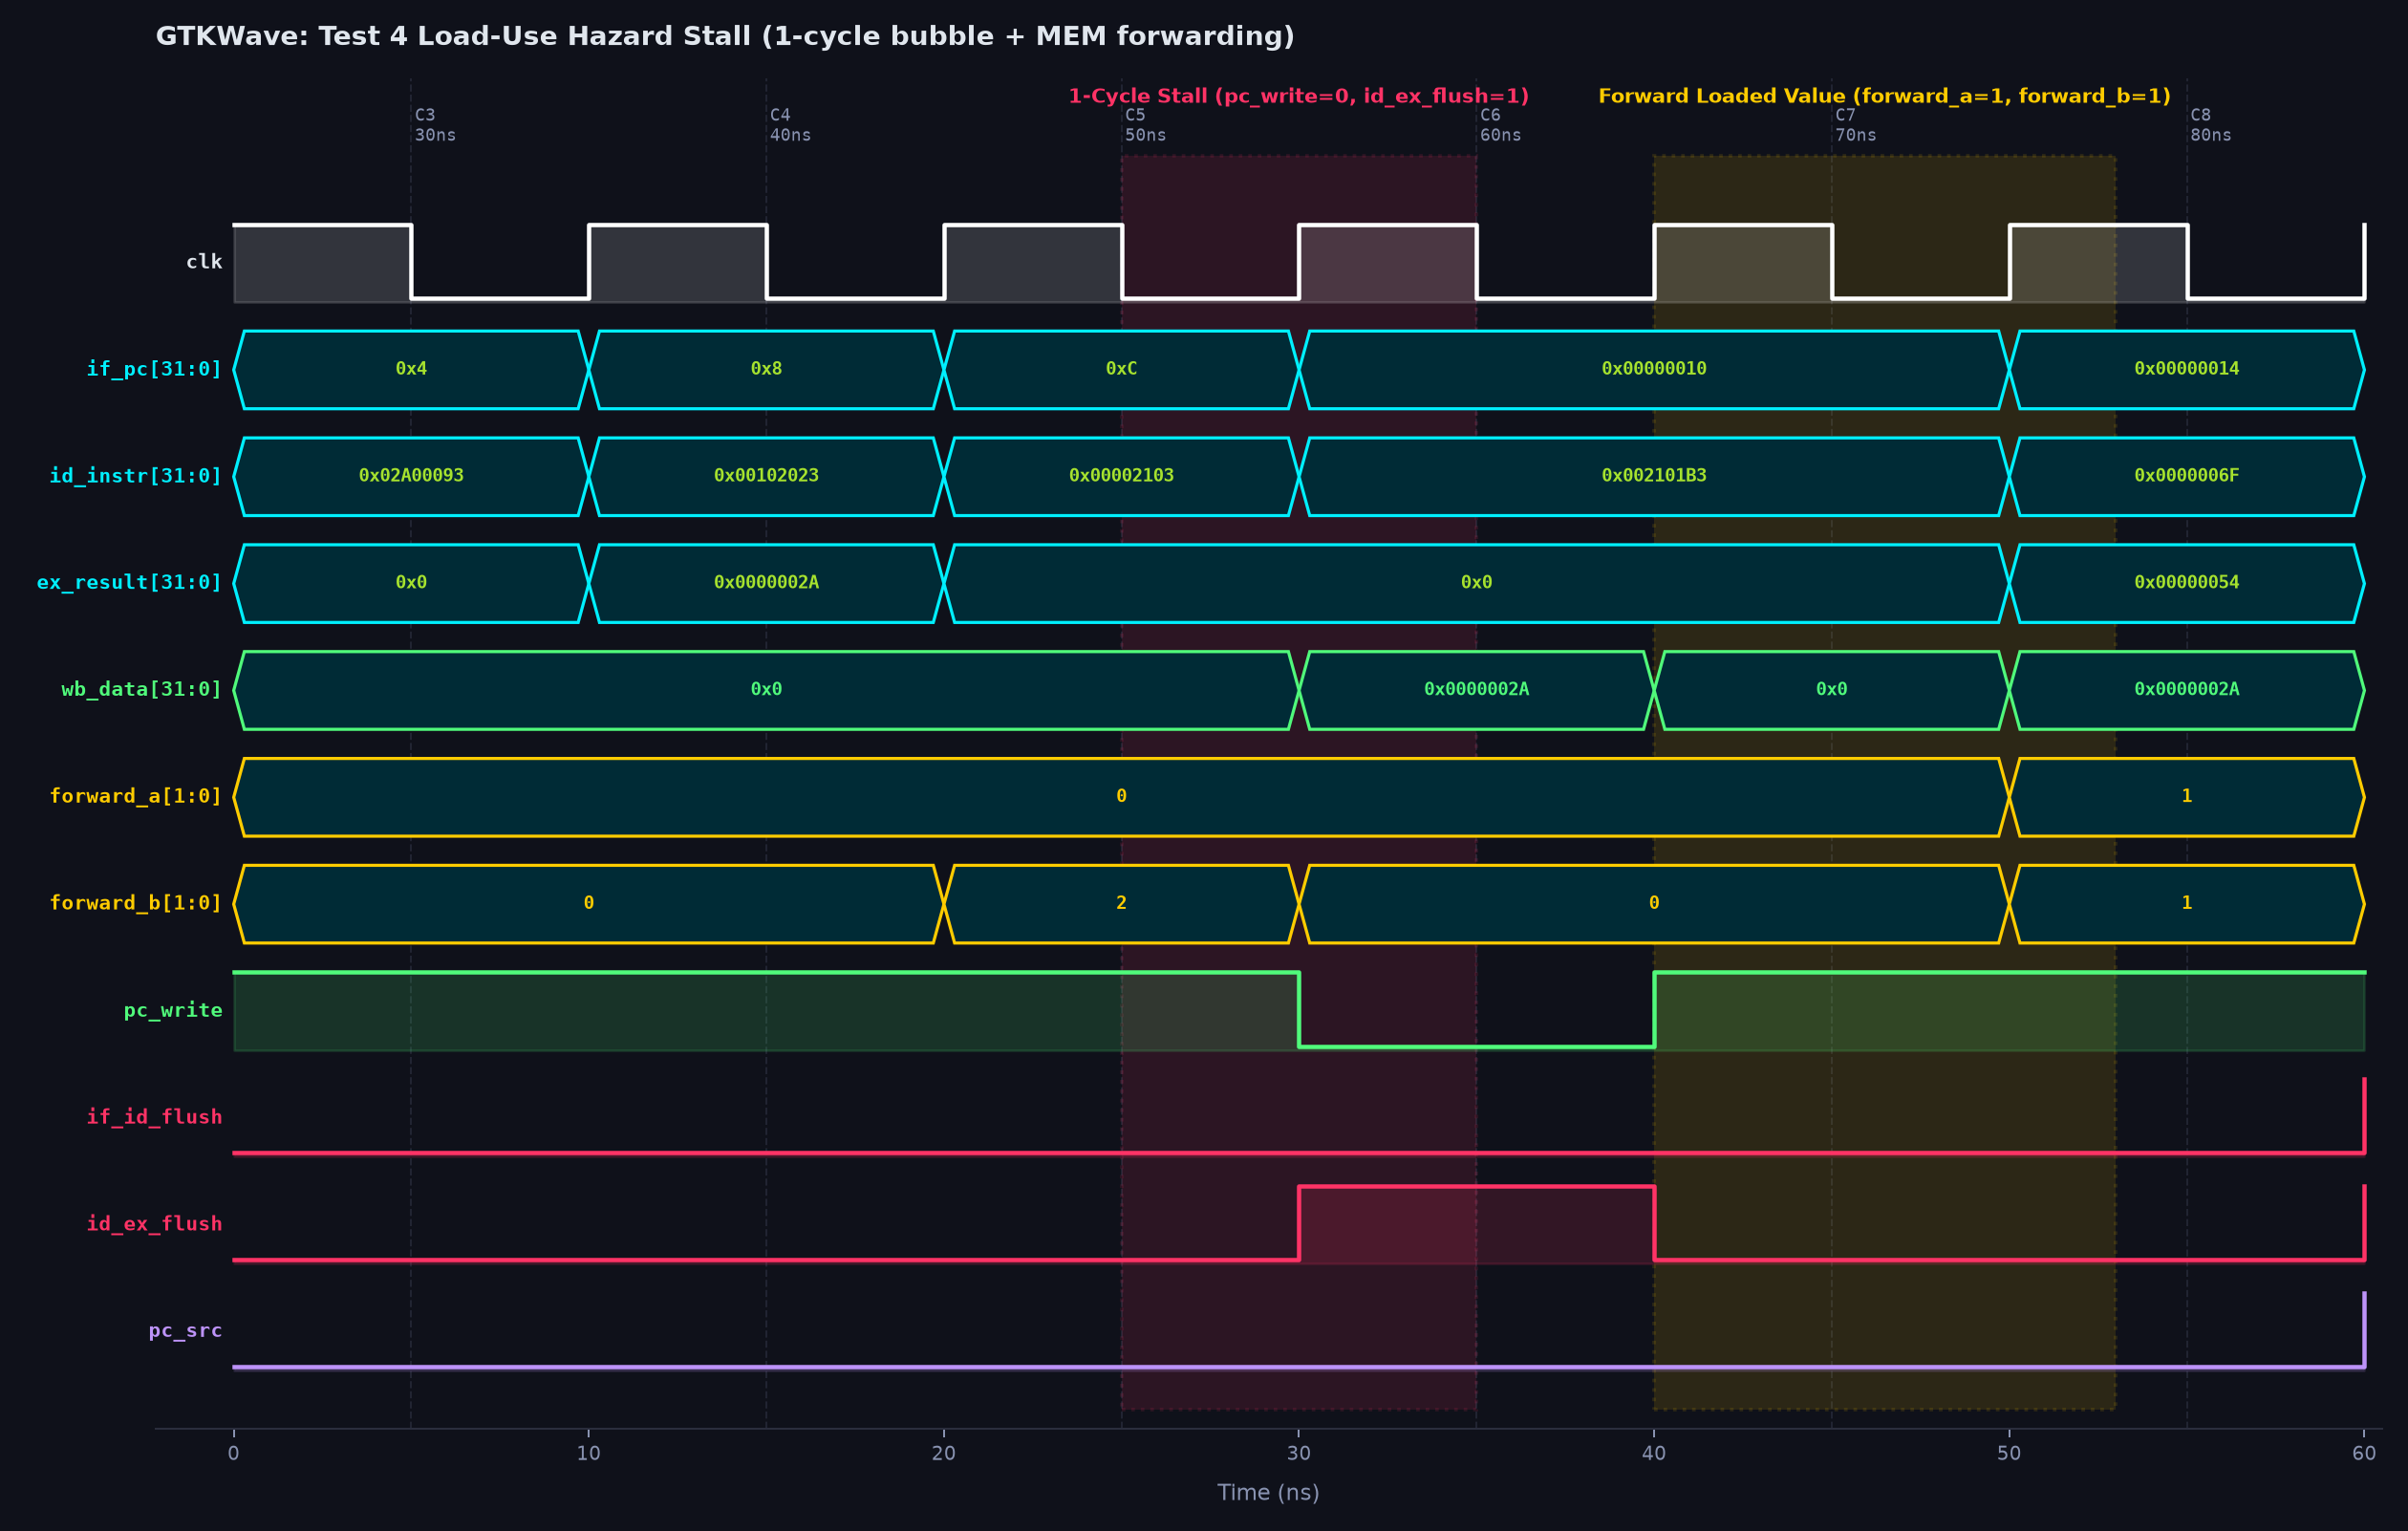
\includegraphics[width=0.92\textwidth]{diagrams/waveforms/load_use_stall.png}
\caption{GTKWave simulation waveform of System Test~4 (\texttt{test4\_loaduse}),
showing the hazard detection unit deasserting \texttt{pc\_write} and asserting
\texttt{id\_ex\_flush} to insert a one-cycle bubble, followed by MEM/WB operand forwarding.}
\label{fig:wave_stall}
\end{figure*}

\begin{figure*}[!t]
\centering
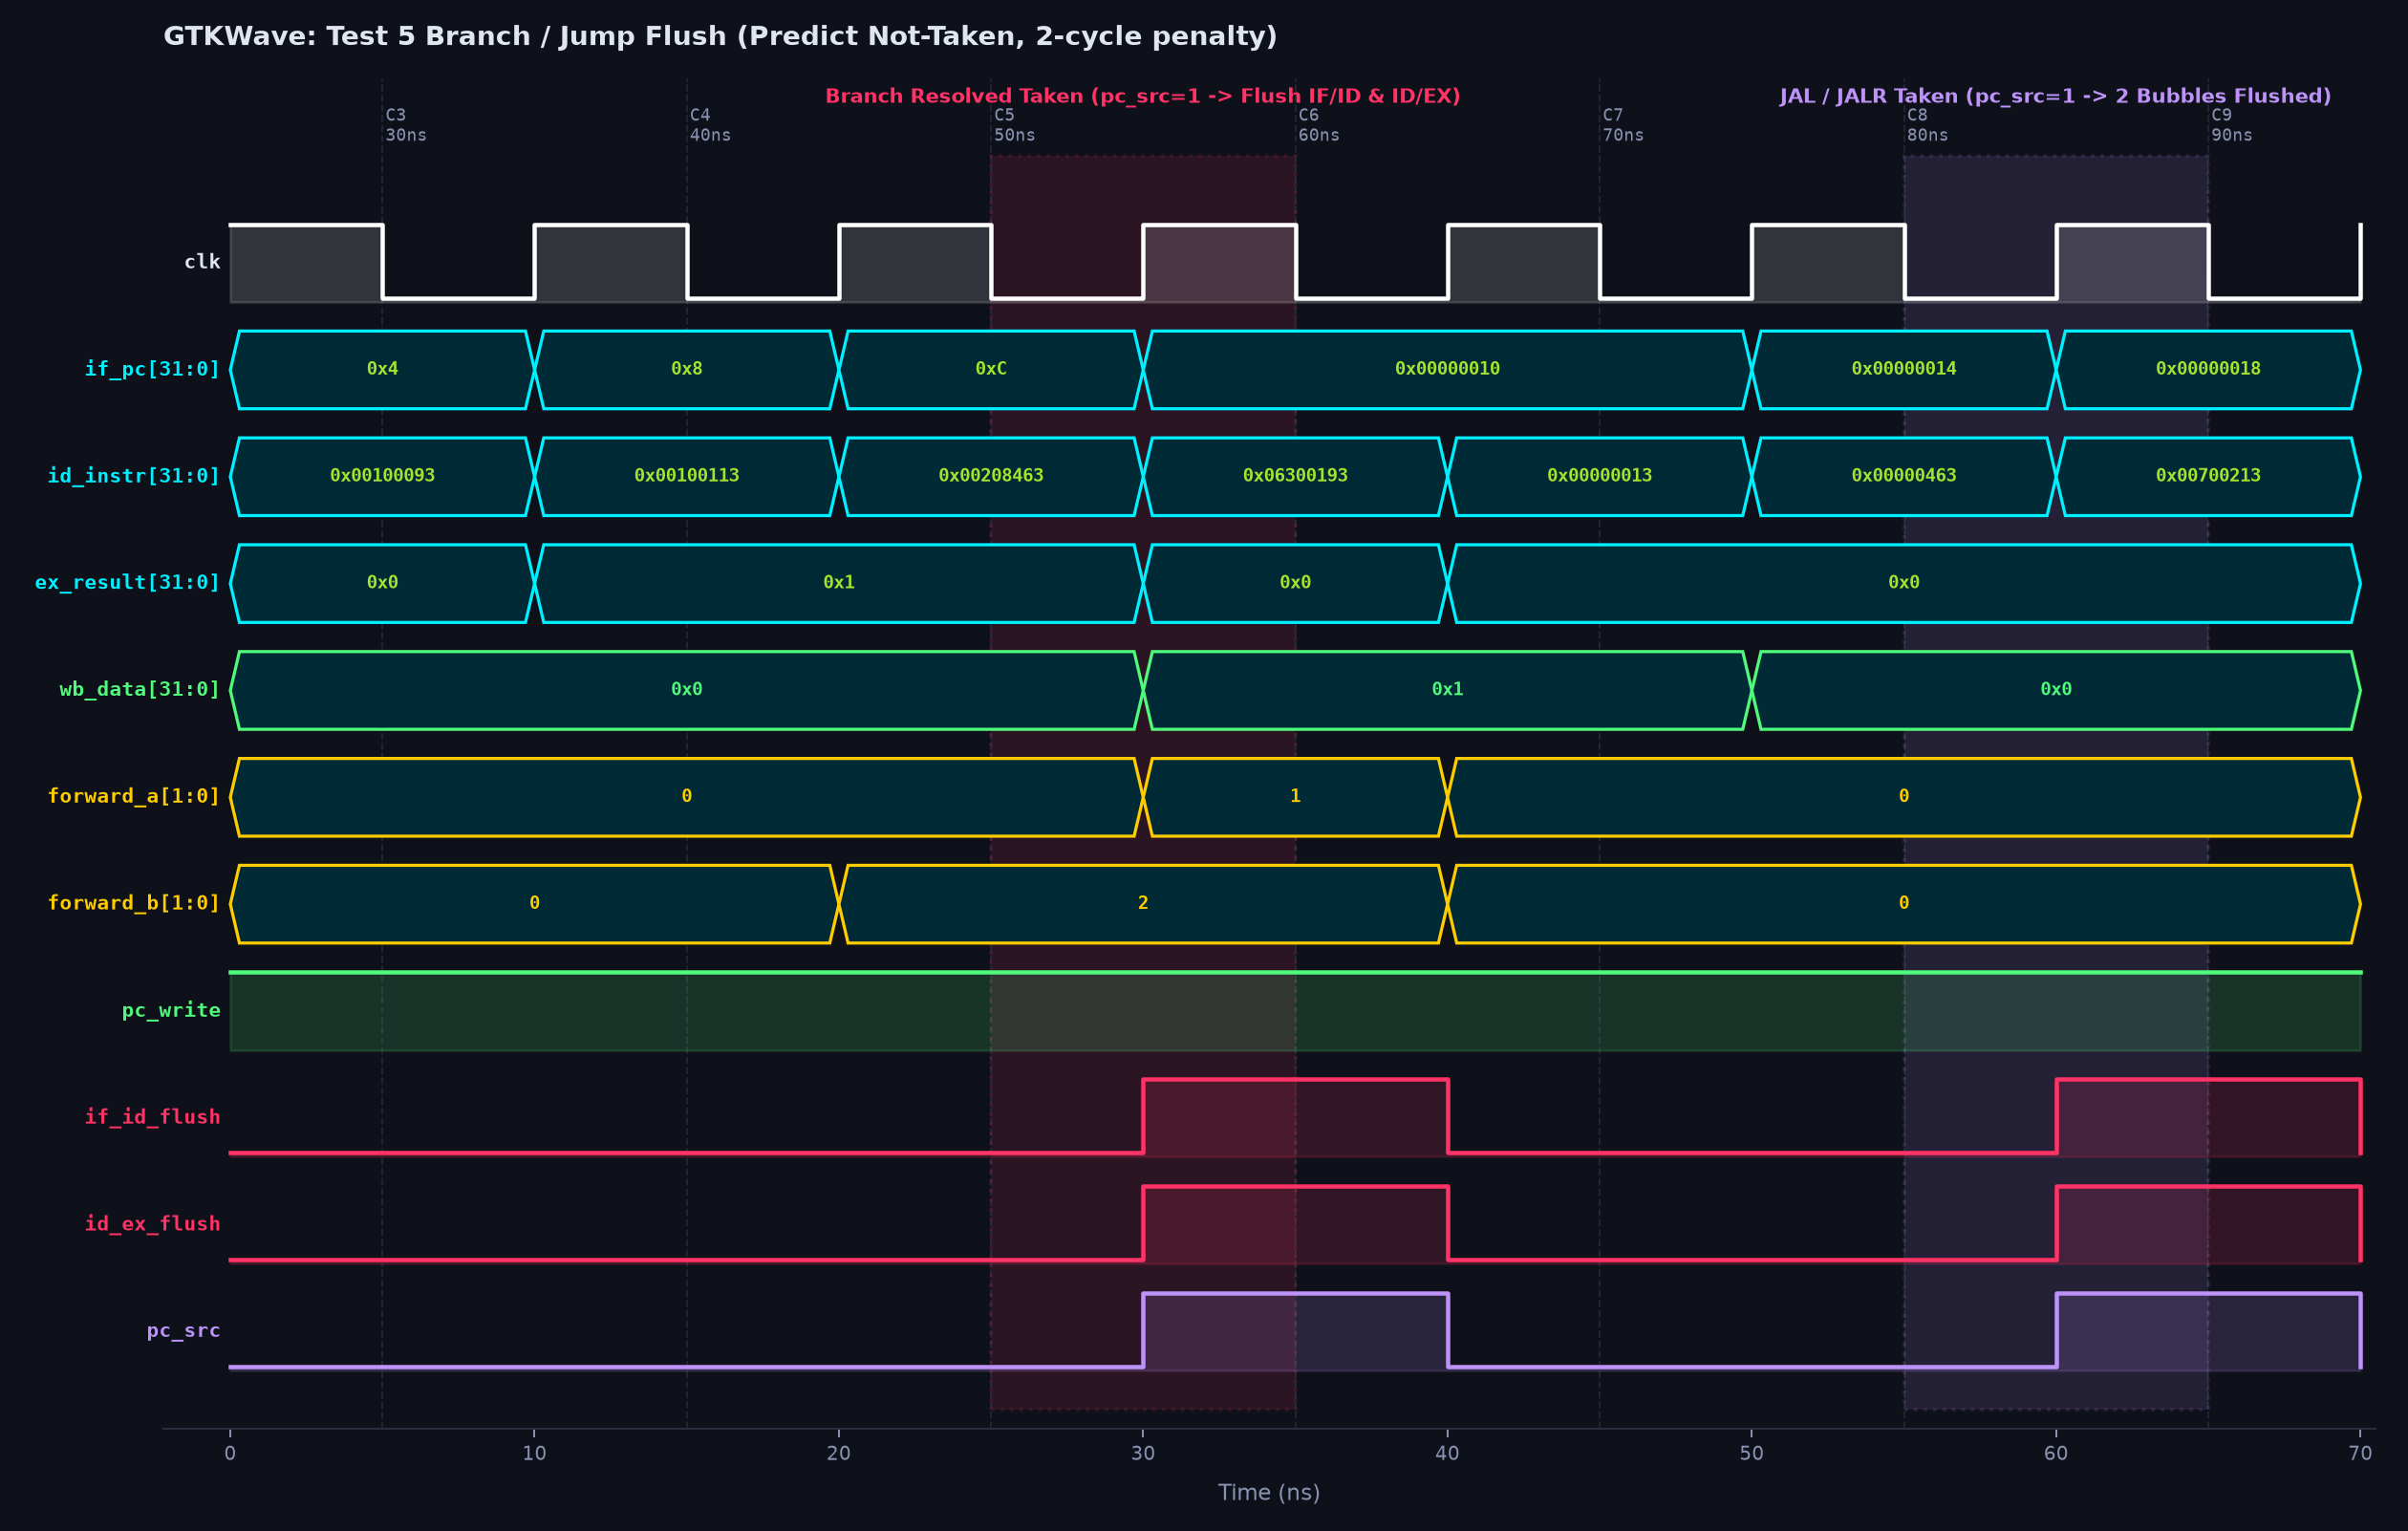
\includegraphics[width=0.92\textwidth]{diagrams/waveforms/branch_flush.png}
\caption{GTKWave simulation waveform of System Test~5 (\texttt{test5\_branch\_jump}),
illustrating branch outcome resolution in the EX stage (\texttt{pc\_src = 1}) and the
simultaneous flushing of two mispredicted instructions (\texttt{if\_id\_flush = 1},
\texttt{id\_ex\_flush = 1}).}
\label{fig:wave_branch}
\end{figure*}

\begin{figure*}[!t]
\centering
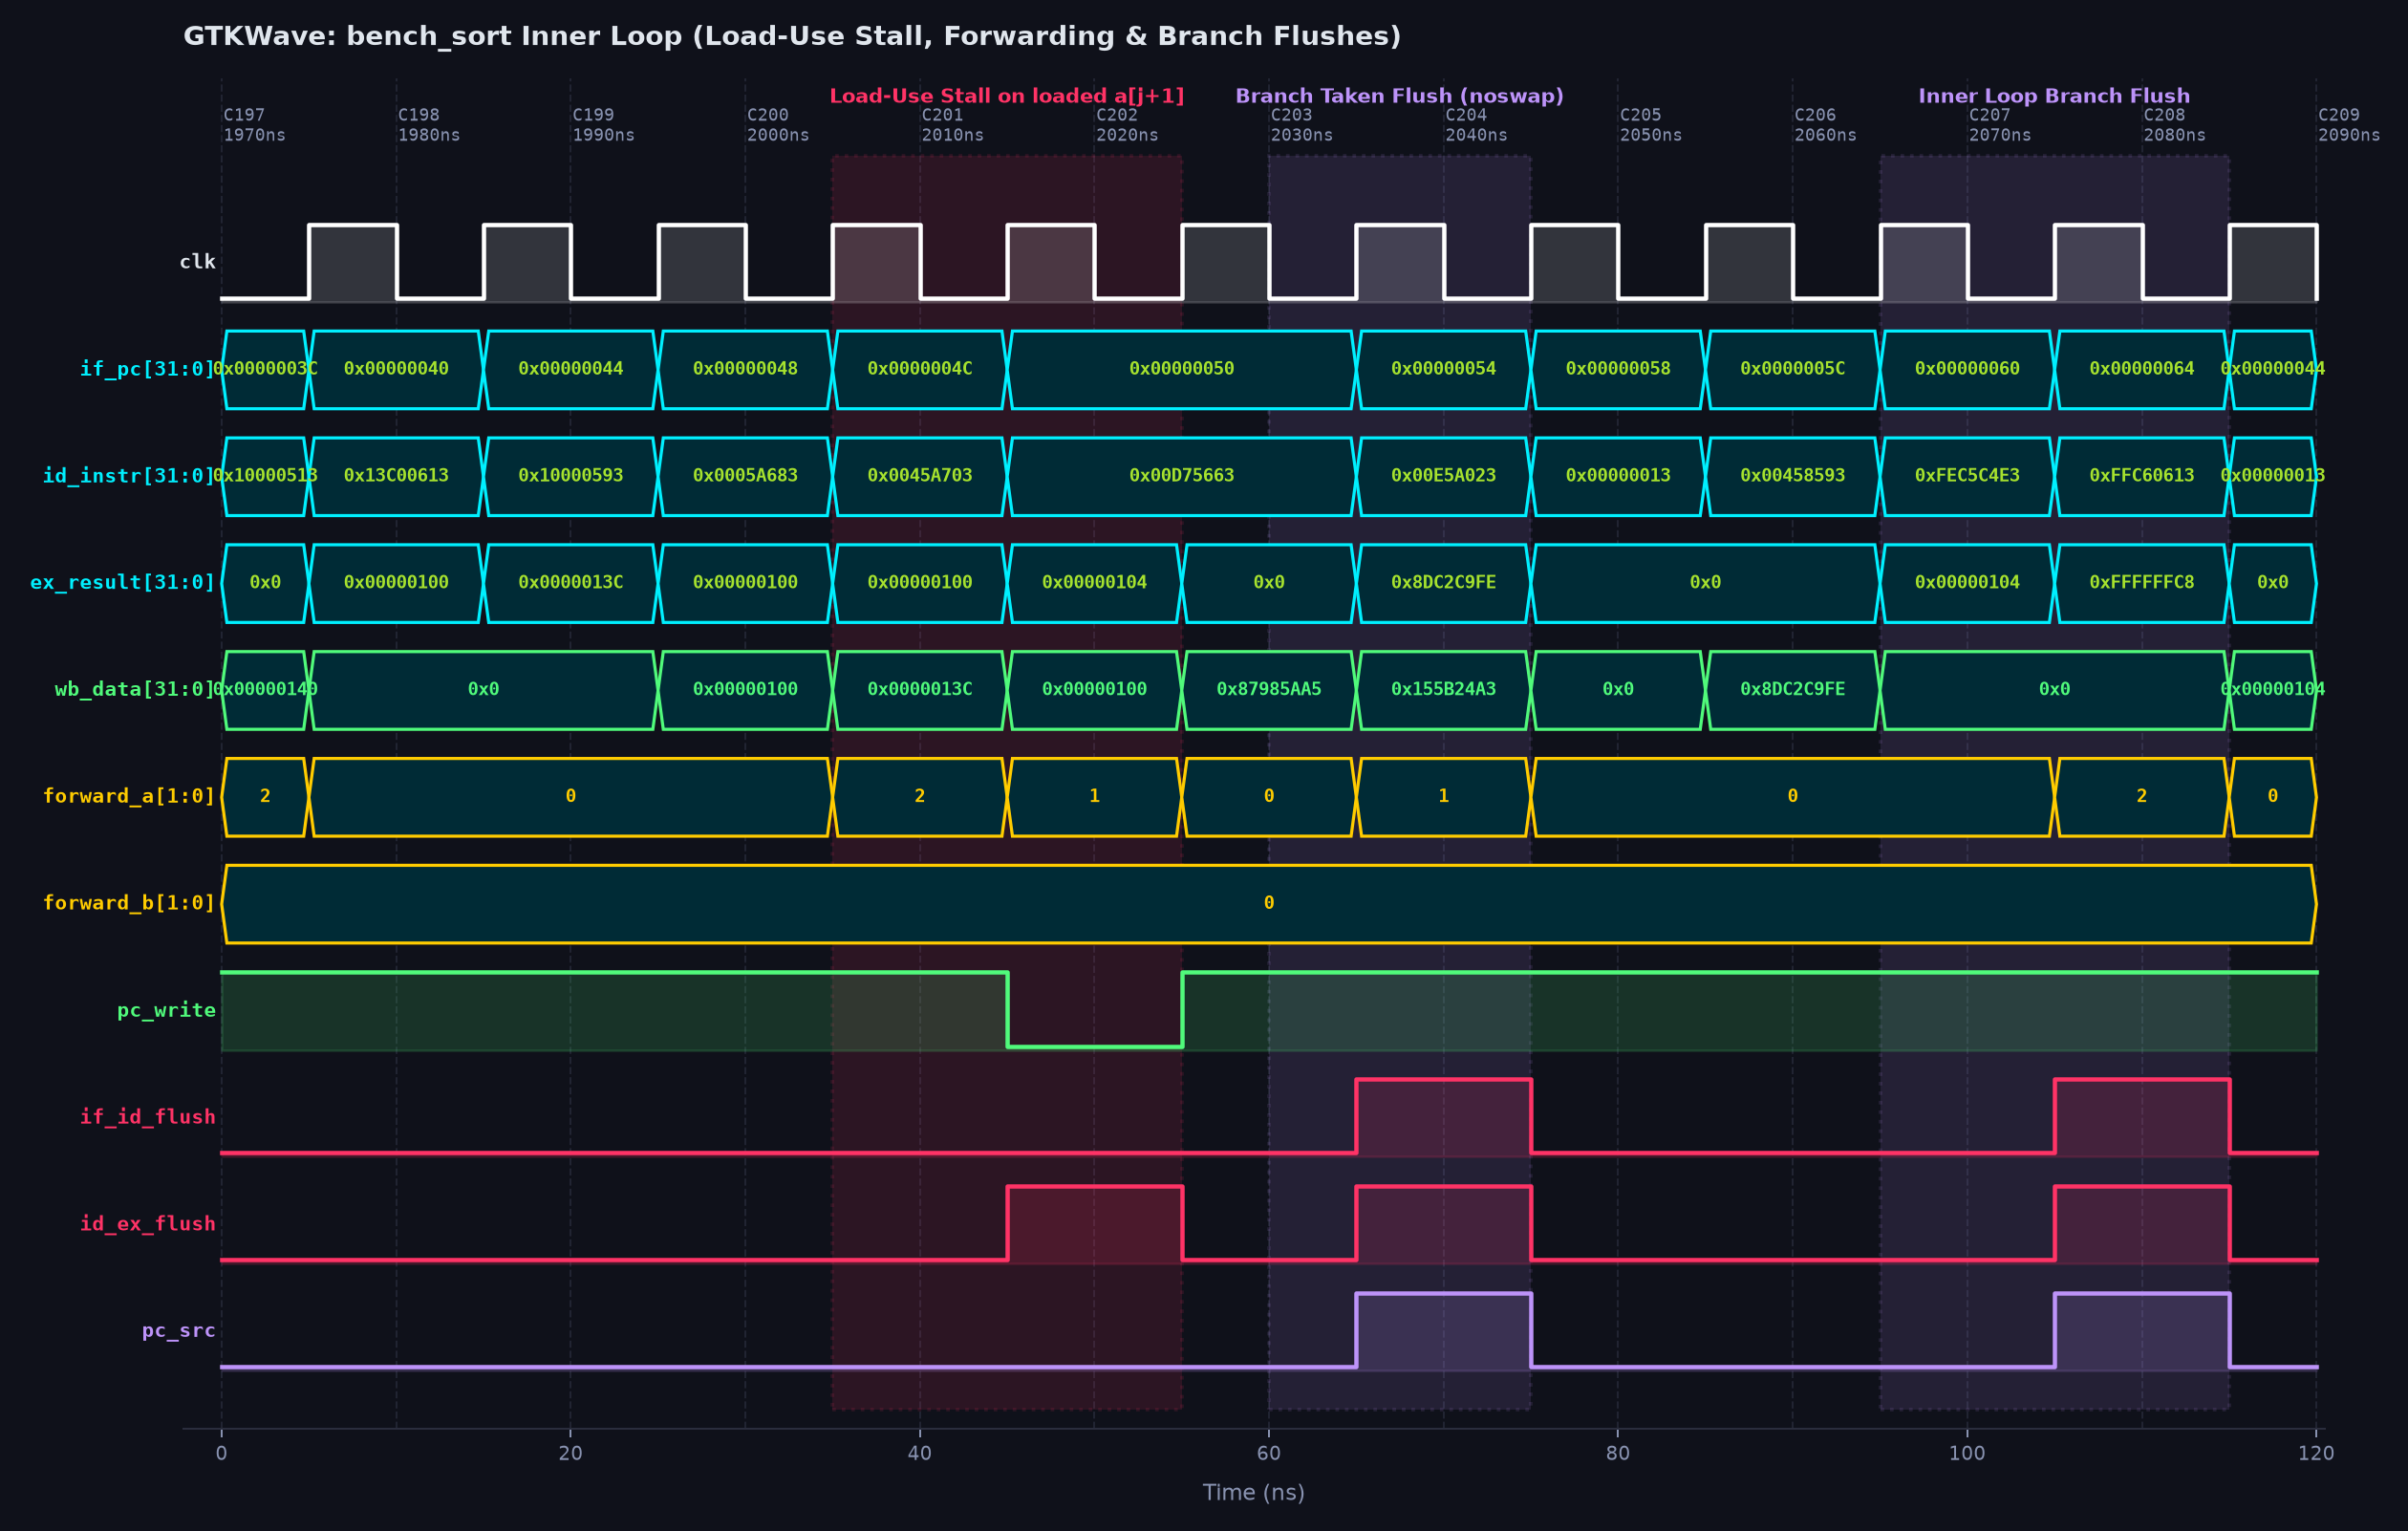
\includegraphics[width=0.92\textwidth]{diagrams/waveforms/bench_sort_loop.png}
\caption{GTKWave simulation waveform of the \texttt{bench\_sort} inner loop (cycles 198--208),
capturing the real-time interaction of load-use stalling, forwarding, conditional branch
evaluation, and loop flushes.}
\label{fig:wave_sort}
\end{figure*}

\paragraph{Data Forwarding (Fig.~\ref{fig:wave_fwd})}
In System Test~3, instruction \texttt{add x3, x1, x2} calculates $10 + 5 = 15$
(\texttt{0x0000000F}) in the EX stage during cycle~4. In cycle~5, the dependent instruction
\texttt{add x4, x3, x1} enters EX. The forwarding unit detects that \texttt{ex\_rs1} ($x3$)
matches \texttt{mem\_rd} ($x3$) with \texttt{mem\_reg\_write = 1}, setting
\texttt{forward\_a = 2'b10}. The ALU selects \texttt{mem\_result} as its first operand,
yielding $15 + 10 = 25$ (\texttt{0x00000019}). In cycle~6, \texttt{addi x5, x4, 1} enters
EX; the forwarding unit again asserts \texttt{forward\_a = 2'b10} from EX/MEM, computing
$25 + 1 = 26$ (\texttt{0x0000001A}) without stalling.

\paragraph{Load-Use Hazard Stall (Fig.~\ref{fig:wave_stall})}
In System Test~4, instruction \texttt{lw x2, 0(x0)} enters EX in cycle~4, followed by
\texttt{add x3, x2, x2} in the ID stage. The hazard detection unit detects that
\texttt{id\_ex\_mem\_read} is asserted and \texttt{id\_ex\_rd} matches \texttt{id\_rs1}
and \texttt{id\_rs2}. In cycle~5, it pulls \texttt{pc\_write} and \texttt{if\_id\_write}
low ($0$) while pulsing \texttt{id\_ex\_flush} high ($1$). This freezes the PC at
\texttt{0x00000010} and holds the \texttt{add} instruction in ID, injecting a NOP bubble into
the EX stage. In cycle~6, \texttt{lw} advances to the MEM stage, and the stalled
\texttt{add} enters EX. By cycle~7, \texttt{lw} is in MEM/WB, and the forwarding unit
selects \texttt{forward\_a = 2'b01} and \texttt{forward\_b = 2'b01}, successfully
forwarding the loaded value ($42 = \texttt{0x0000002A}$) from \texttt{wb\_data} into both
ALU inputs to compute $42 + 42 = 84$ (\texttt{0x00000054}).

\paragraph{Branch and Jump Flushes (Fig.~\ref{fig:wave_branch})}
In System Test~5, instruction \texttt{beq x1, x2, 8} enters EX in cycle~4. Because
$x1 = x2 = 1$, the branch condition is met, and the branch unit asserts \texttt{pc\_src = 1}
and sets the target address to \texttt{0x00000010}. Concurrently, the hazard detection
unit asserts both \texttt{if\_id\_flush = 1} and \texttt{id\_ex\_flush = 1}, purging the
two instructions fetched speculatively under the predict-not-taken assumption
(\texttt{addi x3, x0, 99} and its successor). In cycles~5 and 6, the pipeline executes
the injected bubbles, while IF fetches from \texttt{0x00000010}, incurring exactly the
expected two-cycle flush penalty ($2T$).

\paragraph{Benchmark Inner Loop Execution (Fig.~\ref{fig:wave_sort})}
Fig.~\ref{fig:wave_sort} captures cycles 198 to 208 of \texttt{bench\_sort}, demonstrating
the simultaneous operation of all hazard mechanisms during a bubble sort comparison.
In cycle~200, \texttt{lw x14, 4(x11)} is in EX while \texttt{bge x14, x13, noswap} is in ID.
A load-use hazard is identified, triggering a one-cycle stall in cycle~201. In cycle~203,
the loaded value is forwarded to the branch unit in EX, resolving the branch as taken
(\texttt{pc\_src = 1}). This causes a two-cycle flush of the subsequent \texttt{sw}
instructions, jumping directly to the \texttt{addi} pointer increment. Finally, in cycle~207,
the inner loop test \texttt{blt x11, x12, inner} evaluates taken, branching back to
the next comparison iteration.
